\documentclass[12pt,a4paper,openany]{article}
\usepackage{lmodern}
\usepackage[svgnames]{xcolor} % Required to specify font color
\input{../../LaTexTemplate/templates/couleurs.tex}

\usepackage{makeidx}
\usepackage[utf8]{inputenc} 
\usepackage{marvosym}
\usepackage[T1]{fontenc}
\usepackage[francais]{babel}
\usepackage[top=1.7cm, bottom=1.7cm, left=1.7cm, right=1.7cm]{geometry}
\usepackage{verbatim}
\usepackage[urlbordercolor={1 1 1}, linkbordercolor={1 1 1}, linkcolor=vert1, urlcolor=bleu, colorlinks=true]{hyperref}
\usepackage{tikz} %Vectoriel
\usepackage{listings}
\usepackage{fancyhdr}
\usepackage{multido}
\usepackage{amssymb}
\usepackage{float}
\usepackage[francais]{minitoc}
\usepackage[final]{pdfpages} 
\usepackage{graphicx} % Required for box manipulation
\usepackage{makeidx}

\newcommand{\titre}{FactDev :\\\vspace{10px} Création de devis et facture} 
\newcommand{\titreFooter}{
\includegraphics[width=2cm]{../../../images/FACT_official.png}~~~FactDev : Création de devis et facture} 
\newcommand{\subtitle}{Compte Rendu mensuel : Mois de Février}
\newcommand{\auteur}{Équipe FACT}
\newcommand{\semestre}{~}
\newcommand{\annee}{2015}
\newcommand{\logo}{../../LaTexTemplate/templates/ups.jpg}


\newcommand{\pole}{}
\newcommand{\sigle}{~}
\makeindex
\usepackage[totoc]{idxlayout}


\input{../../LaTexTemplate/templates/listings.tex}
\input{../../LaTexTemplate/templates/article.tex}
\input{../../LaTexTemplate/templates/remarquesExempleAttentionArticle.tex}
\input{../../LaTexTemplate/templates/polices.tex}
\input{../../LaTexTemplate/templates/affichageChapitreArticle.tex}


\newcommand*{\plogo}{\fbox{$\mathcal{PL}$}} % Generic publisher logo
%----------------------------------------------------------------------------------------
%	TITLE PAGE
%----------------------------------------------------------------------------------------

\newcommand*{\rotrt}[1]{\rotatebox{90}{#1}} % Command to rotate right 90 degrees
\newcommand*{\rotlft}[1]{\rotatebox{-90}{#1}} % Command to rotate left 90 degrees

\newcommand*{\titleBC}{\begingroup % Create the command for including the title page in the document
\newlength{\drop} % Command for generating a specific amount of whitespace
\drop=0.1\textheight % Define the command as 10% of the total text height

\vspace*{-50px}
\rule{\textwidth}{0.4pt}\par % Thick horizontal line
\begin{tabular}{p{8cm}p{5cm}p{6cm}}
	\begin{minipage}{8cm}
		Équipe FACT\\
		\textit{Conception et développement d'applications}\\~\\
		\small
%		\Mobilefone~06~84~33~52~93\\
%		\Letter~\texttt{antoine.roquemaurel@gmail.com}\\
		\Mundus~\url{http://fact-team.github.io}
	\end{minipage} &
	& 

	\begin{minipage}{5cm}
		\begin{center}
			
\includegraphics[width=5cm]{logo.jpg}\\
			\tiny{Rédigé avec \LaTeX{}\\Version du \today}
		\end{center}
	\end{minipage}
\end{tabular}

\vspace{\drop} % Whitespace between the top lines and title
\centering % Center all text

\vspace{100px}
\def\CP{\textit{\Huge \titre}} % Title

\settowidth{\unitlength}{\CP} % Set the width of the curly brackets to the width of the title
{\color{LightGoldenrod}\resizebox*{\unitlength}{\baselineskip}{\rotrt{$\}$}}} \\[\baselineskip] % Print top curly bracket
\textcolor{Sienna}{\CP} \\[\baselineskip] % Print title
{\color{RosyBrown}\Large \subtitle} \\ % Tagline or further description
{\color{LightGoldenrod}\resizebox*{\unitlength}{\baselineskip}{\rotlft{$\}$}}} % Print bottom curly bracket

\vfill % Whitespace between the title and the author name


{
\normalsize \LARGE Université Toulouse III -- Paul Sabatier}\\ % Author name

\vfill % Whitespace between the author name and the publisher logo
\Large \today % Year published

\rule{\textwidth}{0.4pt}\par % Thick horizontal line

\endgroup}

%----------------------------------------------------------------------------------------
%	BLANK DOCUMENT
%----------------------------------------------------------------------------------------


\makeatother
\includeonly {
}
\begin{document}
	\thispagestyle{empty} % Removes page numbers
	\titleBC 
	\newpage
	\setcounter{tocdepth}{1}
	\setcounter{secnumdepth}{3}
	
	\tableofcontents
	\newpage
	\section{Le logiciel : FactDev}
	FactDev est un logiciel de Facture \& Devis développé par l'équipe FACT dans le cadre d'un projet de Master à l'Université Paul Sabatier composé de : 
	\begin{itemize}
		\item \textbf{F}lorent Berbie
		\item \textbf{A}ntoine de Roquemaurel
		\item \textbf{C}édric Rohaut
		\item Andriamihary Manan\textbf{T}soa Razanajatovo
	\end{itemize}

	Plus d’informations sur \Mundus~\url{http://fact-team.github.io}

	Notre enseignant tuteur est Frédéric \bsc{Migeon}.

	\begin{figure}[H]
		\centering
		
\includegraphics[width=6cm]{../FACTDev.png}
		\caption{Logo de FactDev}
	\end{figure}

	\section{Période couverte}
	Du 29 Janvier 2014 au 28 Février 2015.

	\section{Résumé des travaux de la période}
	\subsection{Sprint 2}
	Le sprint 2 est composé des \textit{« issues »} préalablement définies et des nouvelles résultant de la première revue de sprint. Ces nouvelles \textit{« issues »} correspondent à des bugs ou des modifications ergonomiques au logiciel. 
	Au niveau du sprint 1 nous pouvions créer un nouveau Client et le modifier. Dans le sprint2, il doit être possible d'ajouter un nouveau projet à un client particulier ou, si le projet existe, de le modifier. A chaque projet d'un client est associé une facture et/ou devis. Ceci engendre des modifications au niveau de l'interface graphique :
	\begin{itemize}
		\item Vue de la liste des clients (existante depuis le sprint 1)
		\item Vue de la liste des projets pour un client
		\item Vue de la liste des factures et/ou devis pour un projet d'un client
		\item Vue hiérarchique avec l'ensemble des clients, ses projets et factures/devis associées
	\end{itemize}
	Afin de s'assurer que l'utilisateur saisi des données correctes on lui empêche de sauvegarder si certains champs sont vide ou erronées. Les champs de saisis possède une icône indiquant la validité ou non des informations qu'ils contiennent. 
	
	\subsection{Sprint 3}
	Le sprint 3 est le dernier de notre première « Release ». La fonctionnalité majeure de ce sprint consiste à créer une nouvelle/facture ou devis avec, pour chacune, les informations suivantes:
	\begin{itemize}
		\item un \textbf{titre}
		\item une \textbf{date}
		\item une \textbf{description}
		\item la \textbf{liste des projets} concernés avec, pour chacun, un tarif (journalier/horaire)
		\item la \textbf{liste des prestations} pour chaque projet avec le nombre d'heures/jours consacrés à la réalisation de chaque prestation
	\end{itemize}
	
	Une fois les informations saisies il est possible de générer la facture au format pdf.
	Dans le cas d'un devis, on doit également pouvoir le modifier ce qui n'est pas le cas d'une facture accessible uniquement en lecture.
	La barre de recherche s'est également améliorée afin de tenir compte des nouvelles modifications, à savoir la possibilité de rechercher par : 
	\begin{itemize}
		\item \textbf{Société} Nom de la société
		\item \textbf{Client} Nom du client
		\item \textbf{Projet} Nom du projet
		\item \textbf{Prestation} Description de la prestation
		\item \textbf{Facture/Devis} Titre ou numéro de la facture ou du devis
	\end{itemize}  
	
	\section{Travaux effectivement réalisés en fin de période}
	L'ensemble des « \textit{issues} » ont été réalisé dans les temps. 
	
	En plus de ce que nous avions initialement prévu, nous avons également réalisé un site internet présentant l'équipe de développement, le projet et
	divers liens propres à ce projet :
	\begin{itemize}
		\item Manuel d’utilisateur : \Mundus~\url{http://fact-team.github.io/doc/usermanual.pdf}
		\item Code source et ressources GitHub : \Mundus~\url{https://github.com/FACT-Team/FactDev}
		\item Documentation :
			\begin{itemize}
				\item Au format HTML : \Mundus~\url{http://fact-team.github.io/doc/html/index.html}
				\item Au format PDF :  \Mundus~\url{http://fact-team.github.io/doc/latex/refman.pdf}
			\end{itemize}
	\end{itemize}

	\section{Charge de travail pour le groupe}
	\subsection{Charge estimé}
	\begin{table}[H]
		\centering
		\begin{tabular}{l|c|c}
			\textbf{Désignation} & \textbf{Fréquence} & \textbf{Total}\\
			\hline
			Réunions tuteur & 1h / semaine & 4h\\
			Réunions de travail & 4h / semaine & 10h\\
			Travail personnel & 8h / semaine & 24h
		\end{tabular}
		\caption{Charge de travail constatée}
	\end{table}

	\subsection{Charge constatés}
	\begin{table}[H]
		\centering
		\begin{tabular}{l|c|c}
			\textbf{Désignation} & \textbf{Fréquence} & \textbf{Total}\\
			\hline
			Réunions tuteur & 1h / semaine & 4h\\
			Réunions de travail & 4h / semaine & 16h\\
			Travail personnel & 8h / semaine & 24h
		\end{tabular}
		\caption{Charge de travail estimée}
	\end{table}
	Nous avions prévu deux heures et demi de réunions de travail avec tout le groupe. Cependant, au début du projet, trois membres du groupes
	connaissaient peu les technologies choisies. Il fut donc préférable de travailler dans la même pièce à la manière d’un « \textit{open space} ». 
	
	Si un des développeurs avait un problème qu'il ne parvenait pas à résoudre, les autres développeurs lui venaient en aide. Ceci contribue à la cohésion
	d'équipe, à la réalisation d’un projet homogène et un avancement plus rapide du projet. 
	
	Cette démarche a aussi été faite dans le but de faire
	progresser rapidement les développeurs afin que ces derniers, ne connaissant pas la technologie, ne bloquent pas sur des problèmes qui sont, pour
	la plupart, mineurs.

	\section{Problèmes techniques constatés}
	\begin{itemize}
		\item Installation de l'outils Sonar
		\item Choix de l'outil tests : QTest a été adopté plutôt que GTest qui posait des problèmes de compatibilité entre les systèmes 
		\item Problèmes de compatibilités entre systèmes : Mac / Windows
		\item Formation sur les technologies
	\end{itemize}
	\section{Décisions prises}
	Avant de rentrer dans le vif du sujet, l'équipe a tenu à mettre en place des standards afin d’assurer une meilleure gestion du projet, une
	meilleure cohésion d’équipe et un code plus homogène. 
	\subsection{La méthode \textit{Scrum}}
	Pour une bonne utilisation de cette méthode, nous avons choisis : 
	\begin{itemize}
		\item Le nombre de versions livrables (\textit{Releases}) et le nombre de \textit{Sprints} par \textit{Release}. Dans notre cas nous avons
			deux \textit{releases} contenant chacune trois \textit{sprints}
		\item Les \textit{User/Technical stories} pour chaque \textit{sprint}
		\item De faire réunions quotidiennes (mêlées)
	\end{itemize}

	\subsection{Utilisation de Github}
	Nous avons rédigés un wiki sur notre compte Github, comprenant :
	\begin{itemize}
		\item Les conventions d’écritures (normalisation des noms de variables, de méthodes, de l'indentation, \ldots)\newline
			\Mundus~\url{https://github.com/FACT-Team/Team-Organization/wiki/Conventions-de-codage-en-C--}
		\item un tutoriel sur Git\newline
			\Mundus~\url{https://github.com/FACT-Team/Team-Organization/wiki/Mini-Tuto-Git}
		\item Un cours explicatif sur notre façon de développer sous Git : une user story aura une nouvelle branche \newline
			\Mundus~\url{https://github.com/FACT-Team/FactDev/wiki/Workflow}
	\end{itemize}

	\begin{figure}[H]
		\centering
		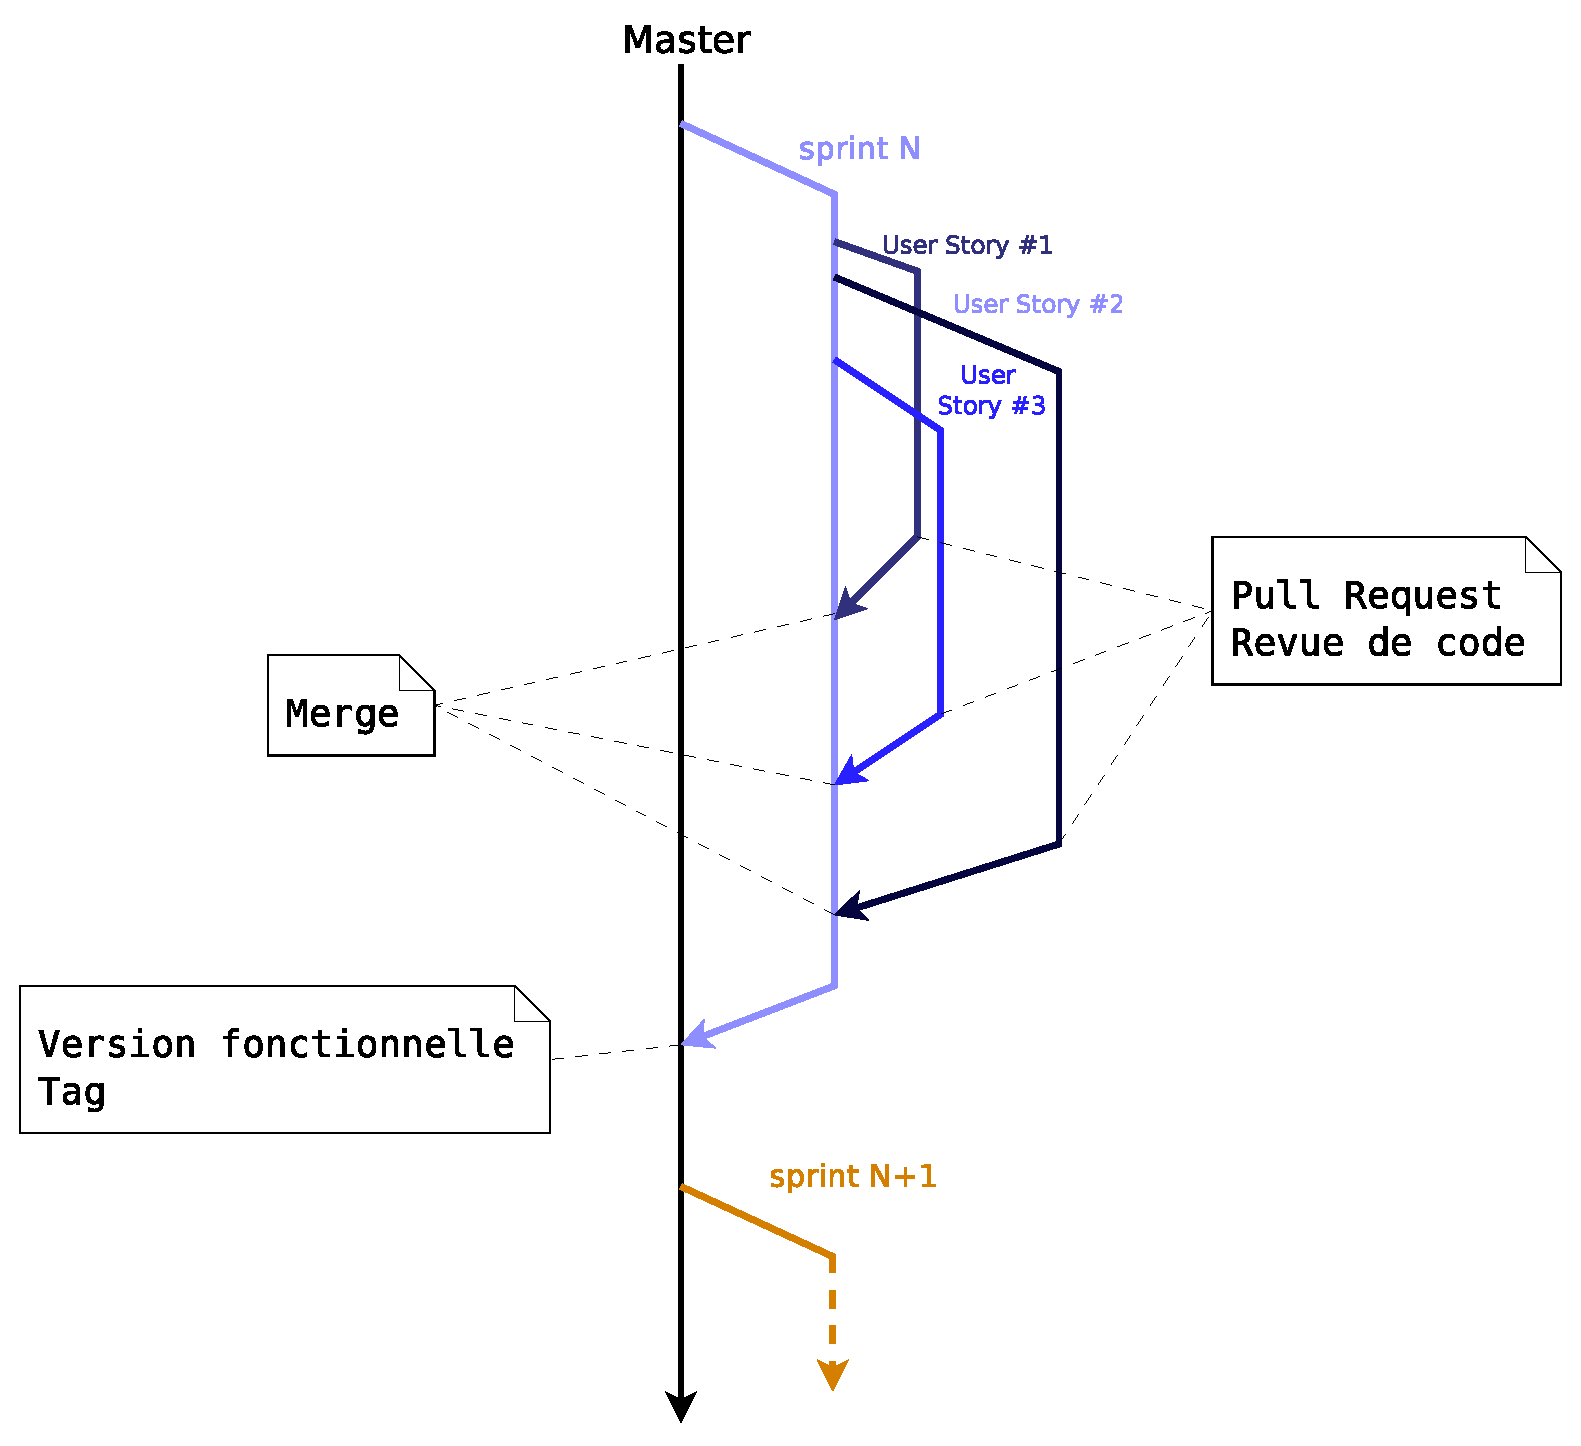
\includegraphics[width=11cm]{BranchingWorkflow.eps}
		\caption{Principe du « \textit{Git Branching Workflow} »}
	\end{figure}
	\subsection{Assurer une revue de code}
	    Le développeur ayant programmé une nouvelle fonctionnalité (et donc créé une nouvelle branche au projet sur Git) mentionne via une <<
		\textit{Pull Request} >> qu'il a terminé.  Les autres membres de l'équipe en sont informés. 
		
		Un de ses membres se charge de la revue de code, ce qui signifie
		qu'il devait vérifier que cela fonctionne et que le code est propre, facilement lisible, peu complexe et commenté. Une fois que tous ces
		éléments ont été revus et jugés valides, la branche est fusionnée à la branche principale (nommée Master) du projet. 

\end{document}
